\documentclass[a4paper,11pt]{article}
\usepackage[a4paper,margin=1in,footskip=0.25in]{geometry}
\usepackage[utf8]{inputenc}
\usepackage{graphicx}
\usepackage{float}
\usepackage{parskip}
\usepackage[style=apa]{biblatex}
\addbibresource{exp.bib}
\usepackage{hyperref}


\title{What challenges are raised by the dissemination and/or communication of knowledge?}
\author{Terry Qi}

\begin{document}

\maketitle

Word Count: 928

Objects:
\begin{enumerate}
 \item The law of demand within my economics book
 \item The bible according to Spike Milligan
 \item Google search result of Fredrick Douglass
\end{enumerate}

\newpage

% Uncertainty
% Context
% Oversaturation

% intro
% This exhibition will explore the prompt by reflecting upon the knowledge within the sciences, more specifically answering whether uncertainty hinder the acceptance and communication of knowledge. While mathematicians often take deductive proofs as granted, this is less common in the area of sciences. Every experiment contains empirical results, but depending on different people with their own personal backgrounds, beliefs, ideologies, or perspectives, the significance of the result will differ between the members of the public. More directly, the lack of trust in the sciences may be a disbelief towards its empirical methods, that uncertainty is untrustworthy and does not bring knowledge.


% knowable thing but could be failified
\subsection*{Object \ref{fig:lod}, The law of demand within my economics book}

\begin{figure}[H]
 \centering
 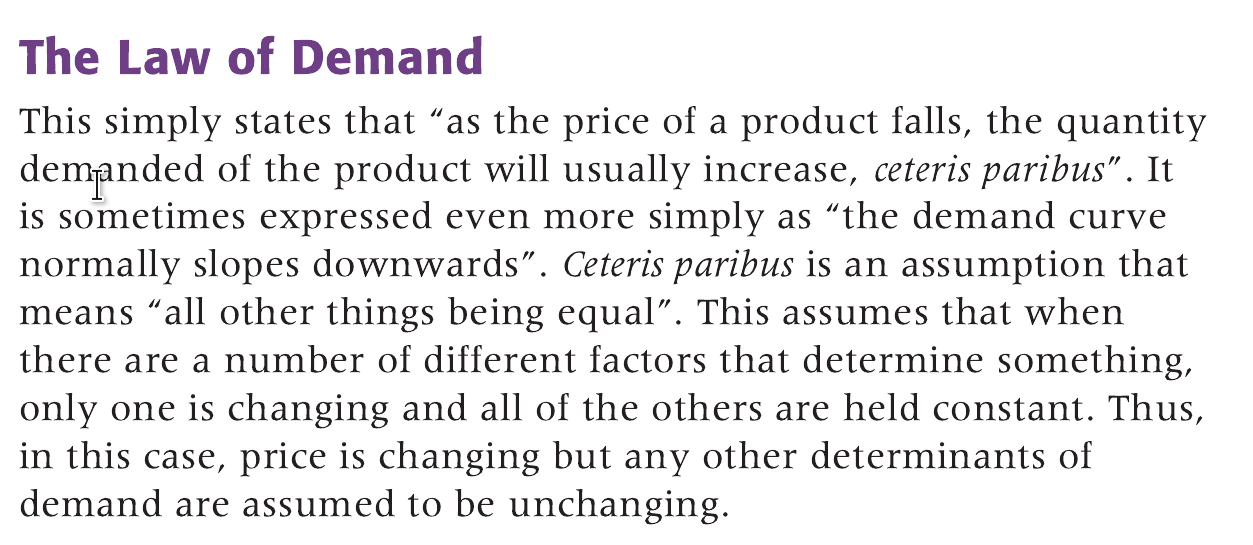
\includegraphics[scale=0.3]{ecobook.png}
 \caption{The law of demand as stated in the book}
 \label{fig:lod}
\end{figure}

This formula comes from my economics course book, stating people's tendency to buy more products when price is lower. This is widely controversial within our class for its inclusion of the word ``law'', and is also attacked globally particularly by psychologists \parencite{DKahneman}, arguing that the theory poses false expectations of human decision making.

The object displays a case where the naming of items can cause challenges in their communication of knowledge.
The use of the word ``Law'' displays certainty on the theory --- arguing the modelling of human behavior to be more knowable than it could be, which often confuses knowers in understanding the theory --- its name is a oxymoron in communicating the assumptions for applying the theory. Coming from a maths background, I did not initially buy into the ``law'' for its vagueness and lack of proof. Additionally, the explanation of the law as shown in the object further complicates this matter by contradicting to the definition of a law: ``a statement of fact'' by using the terms ``often'' and ``usually''. These word send contradictory actions to the knowledge receiver: this is a true fact, and this often happens, thus challenging the exchange of the knowledge.

This object is included in the expedition for it describes how naming challenges the communication of knowledge. In my case, only after a discussion with the teacher and some further research on the topic did I understand how to apply the ``Law''. The object also connects the broad naming errors in the sciences --- naming the existing of charge to be negative. Not only does this harm the understanding of the concepts for beginners, correcting the errors are often very difficult. This showcases the challenge of language in the communication of knowledge as a whole.

% The natural scientists' critique only serves to reveal the flaws in their ``scientific methods'', that the entirety of physics is in essence, fitting numbers to interpretations. While both parties disagrees in acknowledging the shakiness of their disciplines, they are similar in framing the confusion as an ``interesting property'' and a benefit of the sciences, ultimately displaying how the interpretation of empirical evidence differs depending on your personal beliefs and backgrounds.

% context
\subsection*{Object \ref{fig:bible}, The bible according to Spike Milligan}

\begin{figure}[H]
 \centering
 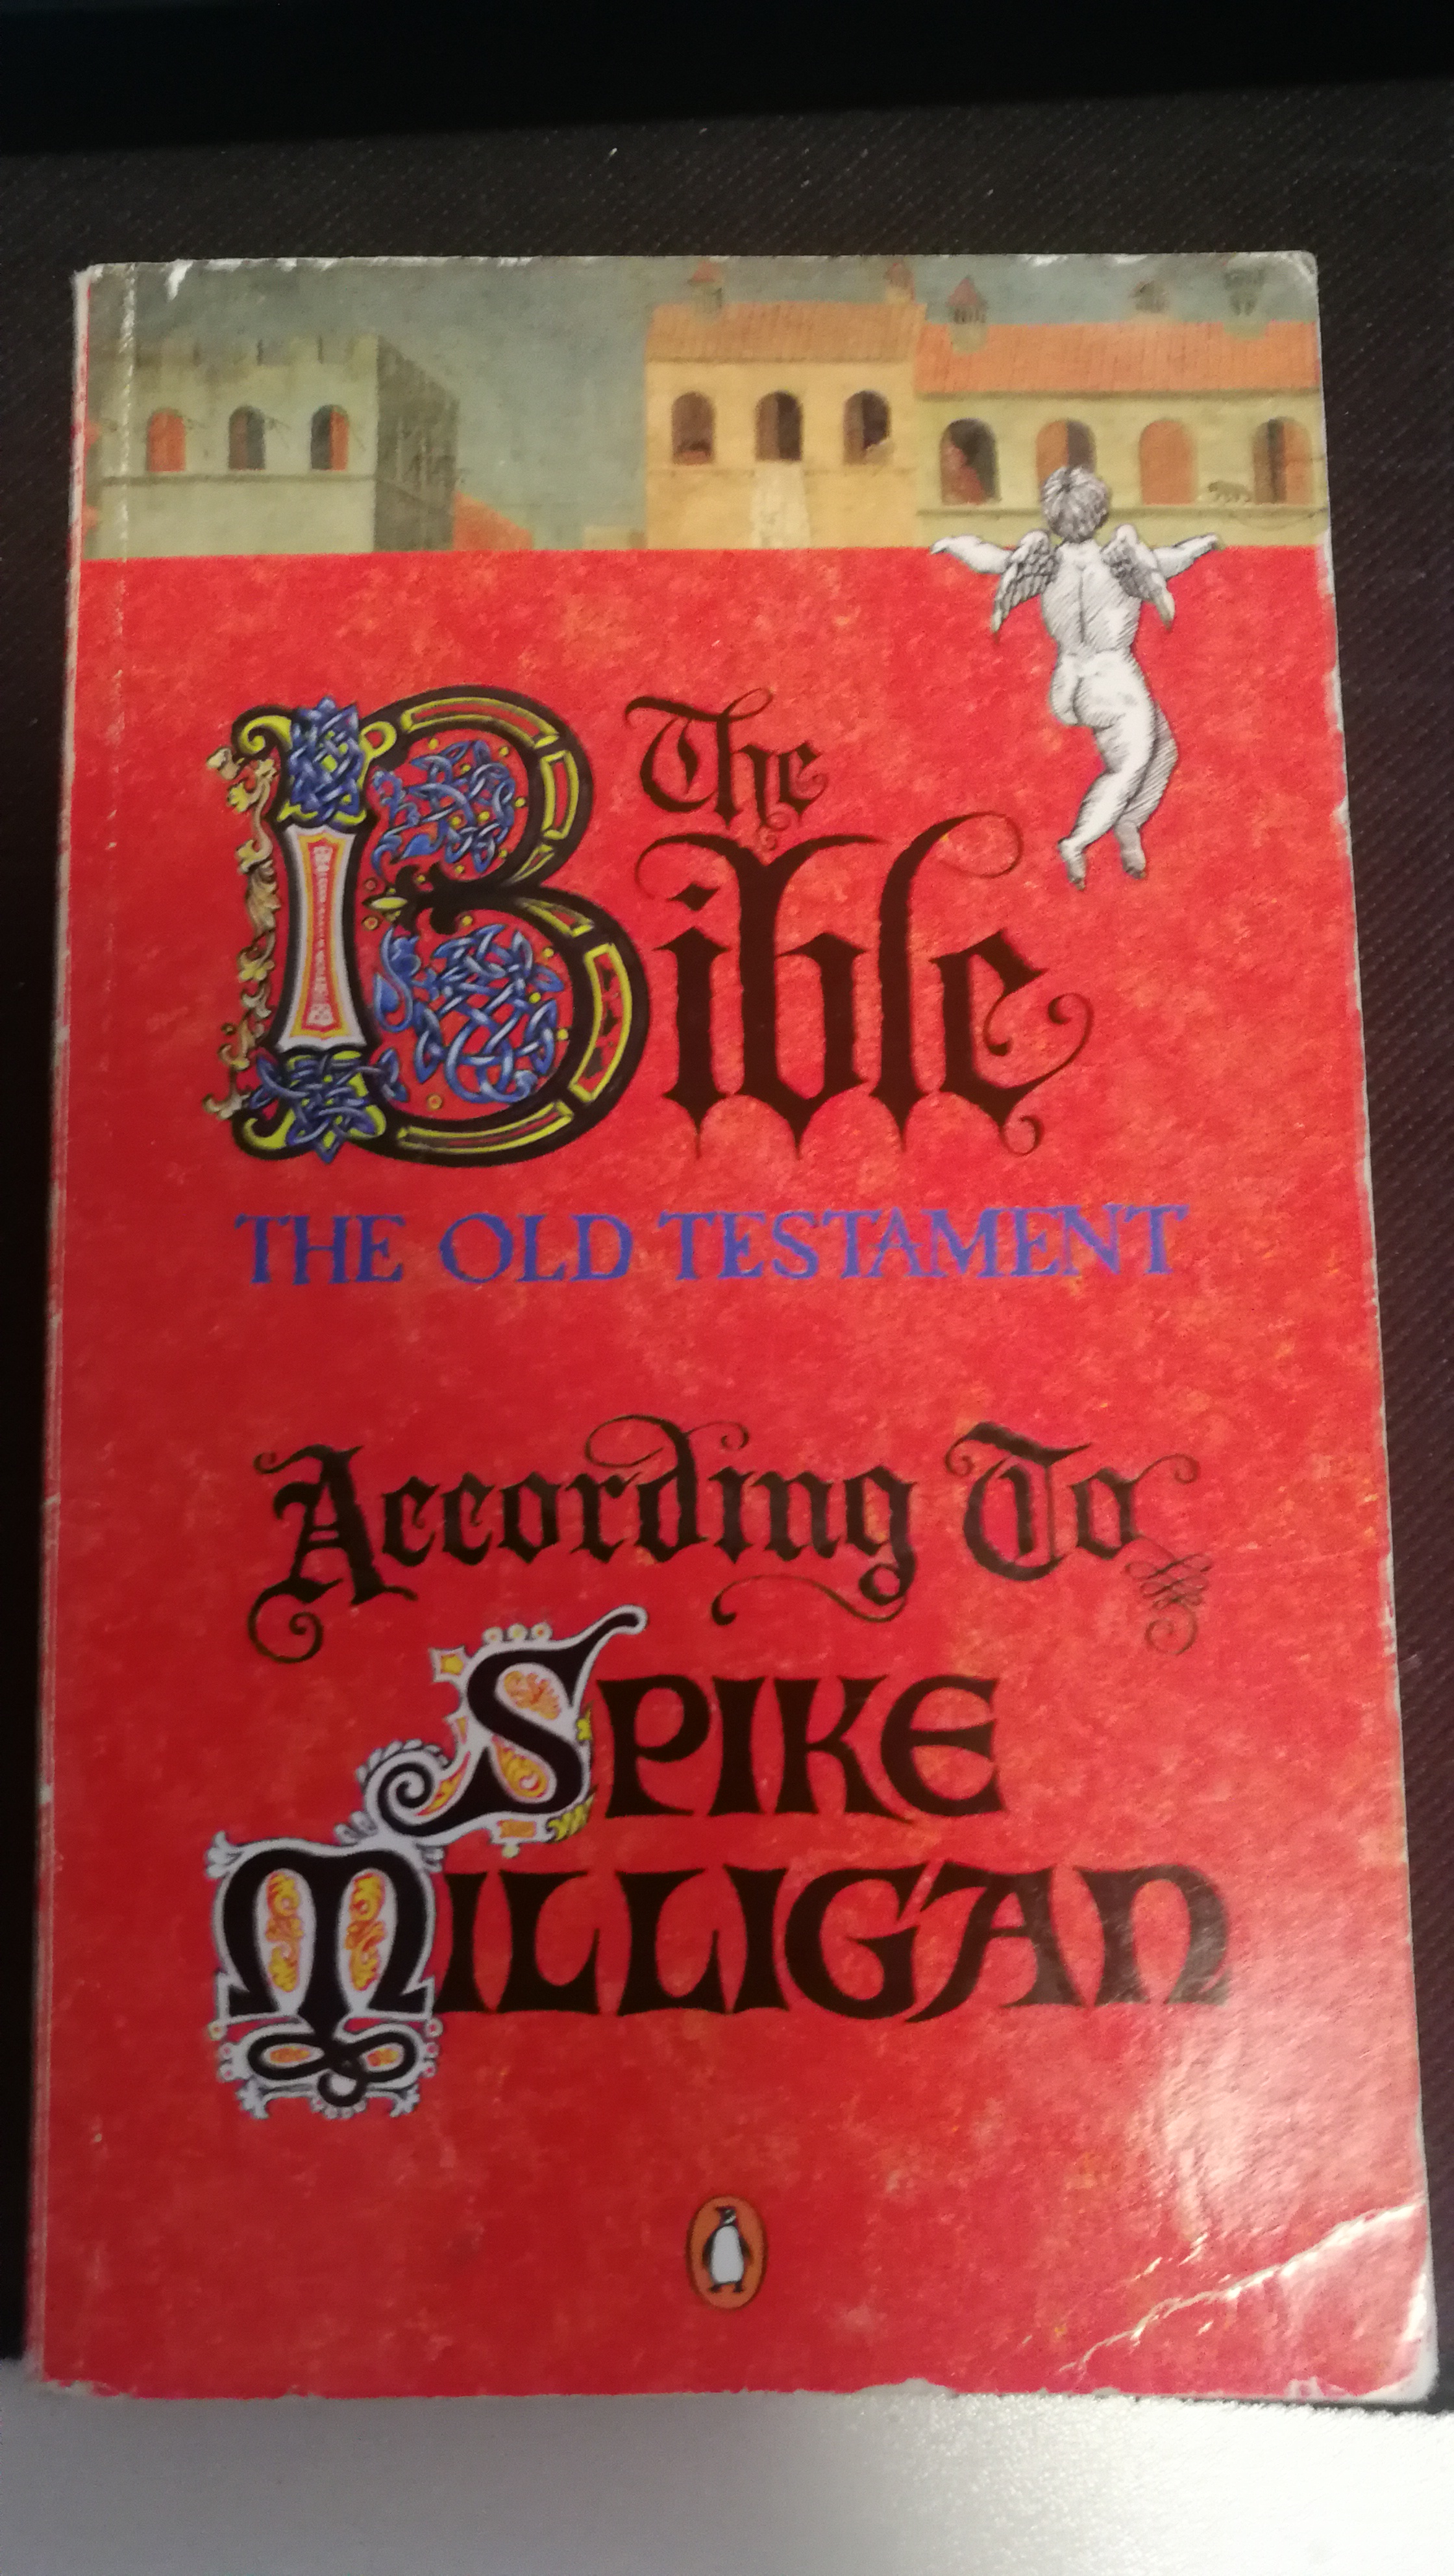
\includegraphics[scale=0.07]{bible.jpg}
 \caption{The bible according to Spike Milligan}
 \label{fig:bible}
\end{figure}

The object is a book issued to me by my friend out of interest, for it parodies the old testament of the bible. The holy bible itself is interesting for its distinctive context 
%--- there are often disagreements on the origin of the bible. Some, and I, use this fact to justify our disbeliefs of the information within the bible. 
--- all of the stories are set in an ancient era. This had deterred me from reading and understanding the book. However, for Spike Milligan had only modified its context while retaining the information the bible held, it is interesting that I find myself enjoying its stories and tales.

The positive personal experience showcases how context can change the ability in the dissemination of knowledge. The existence of a definite context that is set in the modern era helps the reader to visualize the events, which connected to me using modern language and references: such as the mentioning of the GSES test. In contrast with the bible's outdated ancient settings, the object is more easily understood by the modern audience. It also serves to communicate the context of the bible, serving as a base of christian knowledge that I can build upon through my newfound interest on the bible stories. This showcase the importance of context in one's understanding of knowledge, for the parody received even positive reviews online from a mainly non-christian audience \parencite{Review}.

% When people think about the bible, they think of the connection and quotations within it rather than the plausibility and validity of the work. Historically speaking, the bible is special in its unknown origin and writer. Some people view this uncertainty as an argument to reject all meanings within the book, some accepts the knowledge it presents and not by its origin, and some values both interpretations equality.


%The parody of the bible is intriguing for it beautifully shows how the context of its origin can be completely different while retaining its messages and knowledge. The first chapter references the creation of the world, but from a perspective of a British startup firm. Unexpectedly, this shows that the messages of the bible --- that God is took seven days to create the world, is independent of its context, showcasing how the uncertainty of the origin can have little effects on the knowledge presented.

Therefore I included this parody of the bible in the exhibition to be an example where context helps the communication of knowledge. Furthermore, it displays the inevitability of biases in the form of context within the distribution the knowledge, for a single piece of work can be rephrased to appeal to a wider audience. This implies the possibility for knowledge to be distorted or even lost overtime due to context --- a realistic example of a phenomenon of ``Chinese Whispers''.

% Judging from the positive reviews from the various purchasers and I, it seems to display the ability of a common ideology or pure interest to decrease the significance of the context of knowledge. This is in analogy to the ideas presented by the economists --- that the idealistic axioms are justified by a significant result in the knowledge that it creates.


% The object is my personal simulation of some swinging double pendulums. On the surface, it seems that the advances in the natural sciences should be able predict its motions to the atom. But the discovery of chaos questions the fundamental values of physics as a whole. In a sense, some people consider the possibility of uncertainty to be roadblock in the acquiring of knowledge in the sciences.

%Physics as a discipline follows a trend of experiment, theories, and prediction to formulate our understanding of the universe.

% unknowable thing that expresses certainty
\subsection*{Object \ref{fig:download}, Google search result of Fredrick Douglass}

\begin{figure}[H]
 \centering
 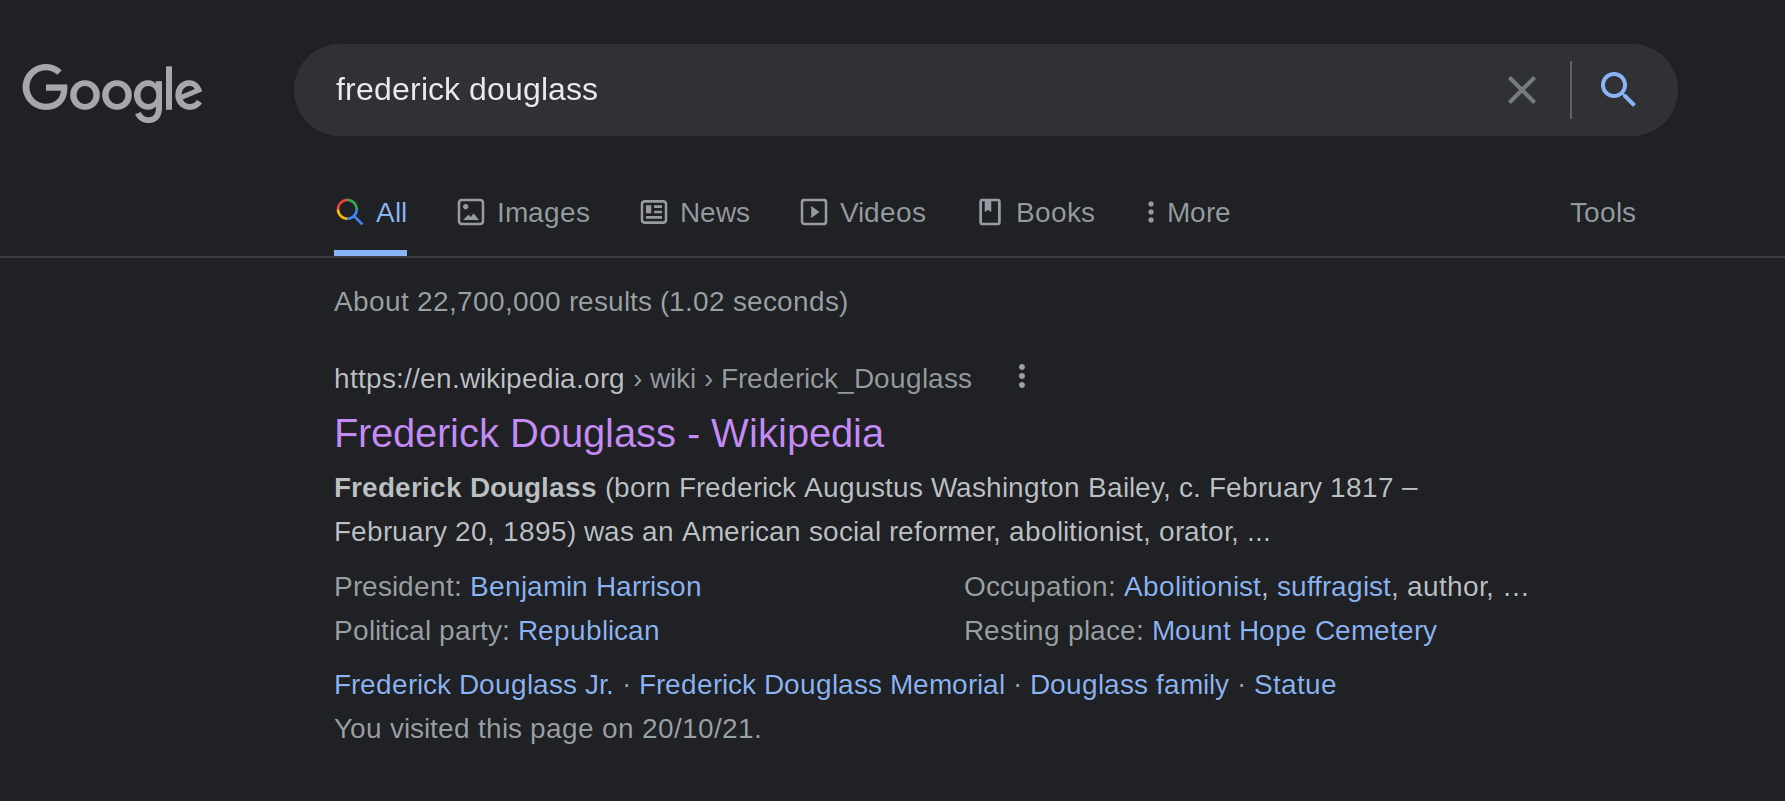
\includegraphics[scale=0.25]{douglass.png}
 \caption{Google search result of Fredrick Douglass}
 \label{fig:download}
\end{figure}

The object here is my personalized Google search result of Fredrick Douglass. The invention of search engines and the internet had brought entire catalogues of encyclopedias to devices that you can hold in your hand. But the easiness of information can also be a challenge in the distribution of knowledge, as one can be overwhelmed with millions of sources (shown in the object with 22 millions results). This often creates a heuristic bias favoring easy information rather than correct information on the internet.

The object have the website Wikipedia as the top result, which displays the internet's effects on the sharing of information online. The ordering of knowledge sources limits the reach of other lesser popular knowledge sources further down the page, as the average viewer is likely to select the first result. This creates a challenge in the dissemination of knowledge with a bias towards popular sources. The single source of information narrows the scope of human knowledge --- students often conduct research based on Wikipedia alone, and I have heavily relied on this page for my English research and didn't bother finding other perspectives on his life. It shows how people lose decision making abilities in their selection of information on the internet as a consequence of the masses of knowledge available online, causing most events to be only seen from one side of the argument.

 %People in the 21st century would often pick the most visible and easiest route to get information and knowledge on a subject, creating a bias towards a single source of truth stemming from the effects of an oversaturation of knowledge.

The importance of the internet at the modern age justifies this object's position in my exhibition. Its statistics on the number of results made me realize the true difficulty in understanding a topic from all views on the internet, which poses a challenge for me to find all the perspectives on the speaker. Moreover, the sea of information on the internet may imply a future where knowledge does not exist, a world full of only opinions and persuasive writings due to the laziness and inability for humans to check all trillion sources on a single war, displaying the hypothetical peek of the challenges in the communication of truth. Sometimes in life, the less decisions the better, and the less information, the more meaningful they are.

%The object is a progress bar of a file download in the my Firefox browser. It have the purpose of displaying the time it takes to download this very important file I need. This sight had only became more common in the information era, yet it had surprised me to know that the underlying progress it displays has no certainty. The progress bar serves as a distraction to the nondeterministic information of file downloading for the user.

%While this little bar can come in many forms, there exist an endless flow of people complaining the inaccuracy of the device, yet the purpose of the device is for good --- to create feedback upon an action. It implies the idea that covering uncertainty with certainty, where knowledge is deliberately hidden, is undesirable to people. Additionally, versions of progress bars which does not cover the uncertainty does not escape the criticisms. It seems to me that people fear the concept of covering uncertainty with certainty, showcasing inability to reduce uncertainty in the communication of knowledge.

%The common appearances (and criticisms it faces) of the item helps in broadening the scope of the knowledge question. The progress bar showcases the general knower's desire for information in the event of a knowledge barrier, and its fear for the censoring of knowledge. For I have made progress bars myself in my apps, I find the understanding of the underlying knowledge the bar covers --- whether uncertain or not, helps in reducing the frustration of such a progress bar. This showcases the ability of uncertainty, even if covered with certainty, to induce frustration and communication of knowledge.

\nocite{*}
\printbibliography


\end{document}
